\section{WebGL and OpenGL standard}\label{webgl-and-opengl-standard}

\subsection{Evolving of the standards}\label{evolving-of-the-standards}

The publication and draft dates of WebGL specification:

\begin{itemize}
\tightlist
\item
  Version 1.0, 10 February 2011
\item
  Version 1.0.1, 27 January 2012
\item
  Version 1.0.2, 01 March 2013
\item
  Version 1.0.3, 27 October 2014
\item
  Version 2.0, 19 February 2016 (latest draft)
\end{itemize}

NOTE: Version 1.x are based on OpenGL ES 2.0; Version 2.x are based on
OpenGL ES 3.0.

NOTE:The 2.0 draft spec
\href{https://www.khronos.org/registry/webgl/specs/latest/2.0}{provided
here} should be read as an extension to the WebGL 1.0 specification. It
will only describe the differences from 1.0.

\subsection{Information in the
standards}\label{information-in-the-standards}

\subsubsection{WebGL}\label{webgl}

In \href{https://www.khronos.org/registry/webgl/specs/latest/1.0/}{WebGL
spec}, it introduces \emph{Context Creation} and \emph{Drawing Buffer
Presentation}, \emph{WebGL Resources} and \emph{Security} only briefly.
The major parts are: \emph{DOM Interfaces} and \emph{Differences with
OpenGL ES 2.0}.

In DOM interfaces, the types and various object interfaces are
introduced, in which the \texttt{WebGLRenderingContext} is the biggest
one. The IDLs are presented here, and its intended semantics are
described. However, it refers OpenGL ES 2.0 frequently and don't give a
lot of information which appears in the OpenGL spec.

Here is a sample spec:

\begin{figure}[htbp]
\centering
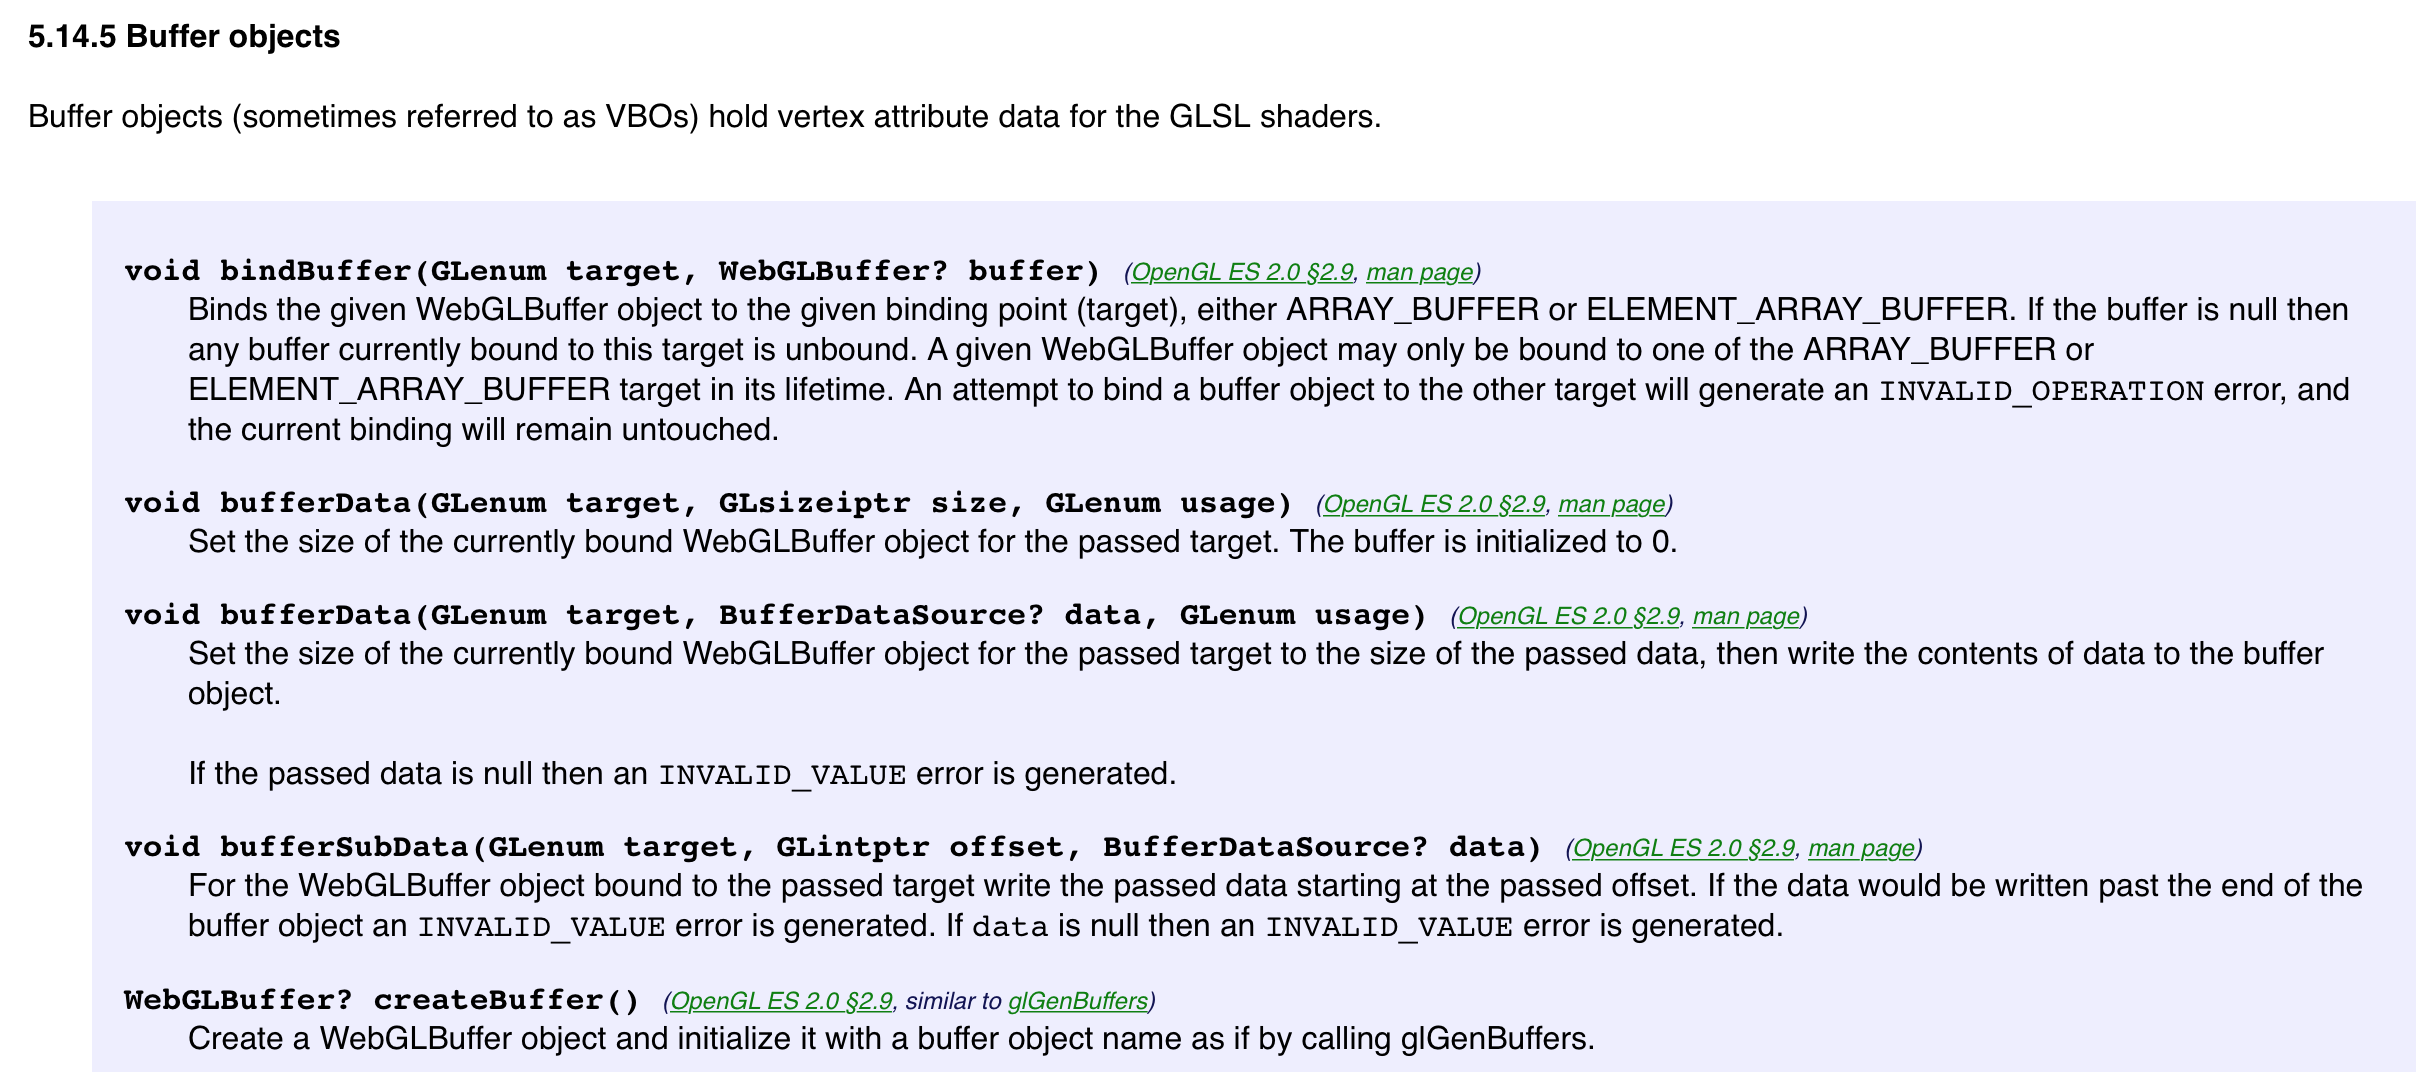
\includegraphics{webgl-spec.png}
\caption{}
\end{figure}

\subsubsection{OpenGL ES}\label{opengl-es}

The
\href{https://www.khronos.org/registry/gles/specs/2.0/es_full_spec_2.0.25.pdf}{OpenGL
ES 2.0 spec} is a rather detailed specification. Some implementation
contrives are explained. So it is necessary for understanding the
browser implementation.

Here is a sample spec:

\begin{figure}[htbp]
\centering
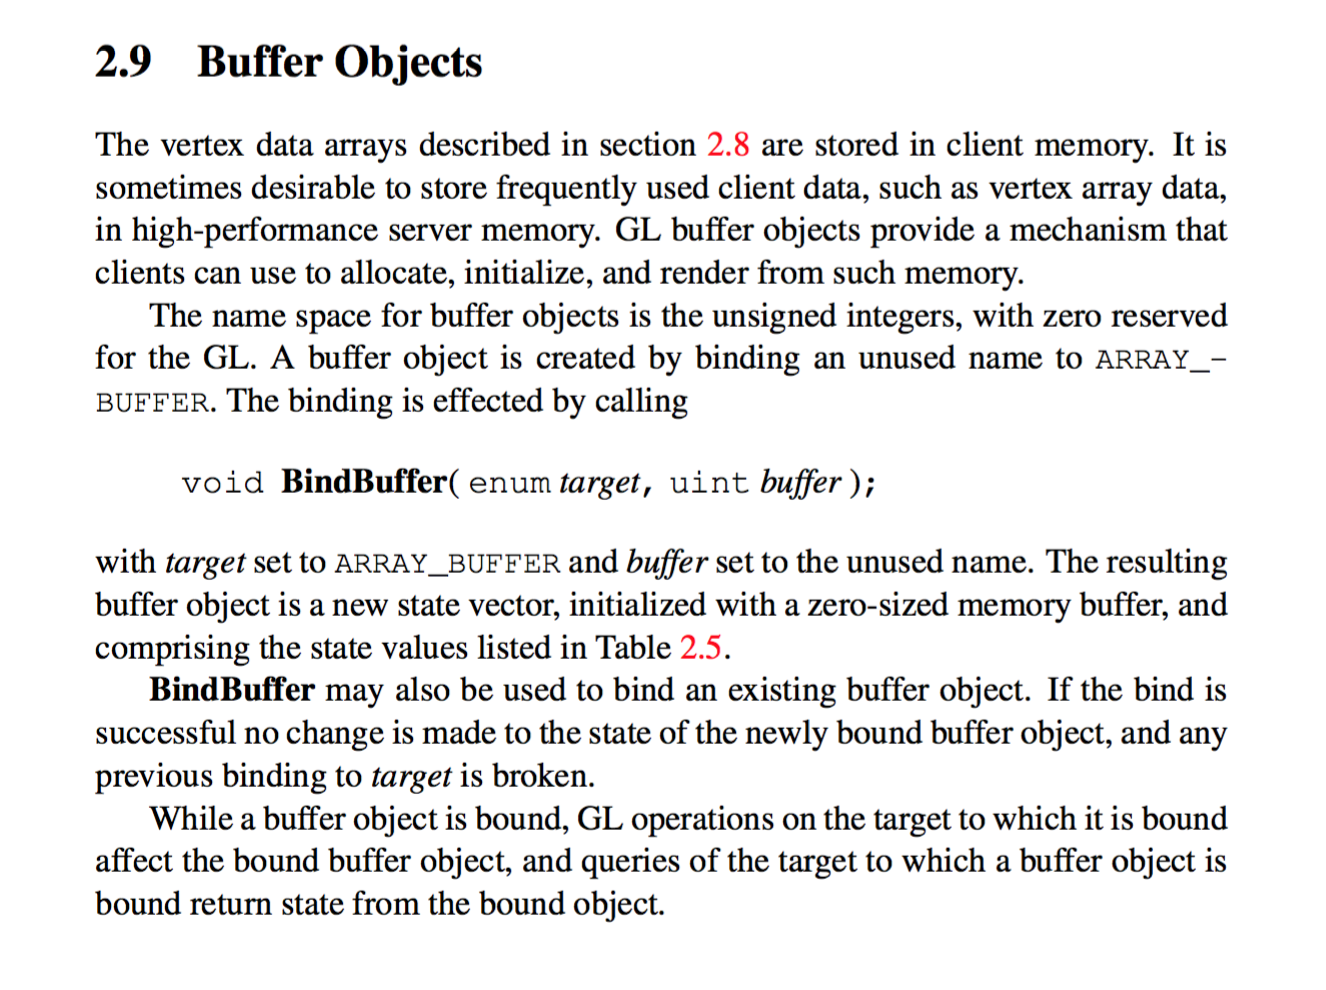
\includegraphics{opengl-spec.png}
\caption{}
\end{figure}

\subsubsection{Example Implementation}\label{example-implementation}

As an example of implementation, we will see part of code in Firefox's
Browser Engine -- Gecko.

\begin{itemize}
\tightlist
\item
  \href{https://github.com/mozilla/gecko-dev/blob/5a7da7930ebba958d98e2e42ed07d05c34d1873a/dom/webidl/WebGLRenderingContext.webidl}{\texttt{WebGLRenderingContext.webidl}}
\item
  \href{https://github.com/mozilla/gecko-dev/blob/71900c9741a8fafb137d9a57519dfa0fe280c4dc/gfx/angle/src/libANGLE/renderer/gl/RendererGL.h}{\texttt{RendererGL.h}}
\item
  \href{https://github.com/mozilla/gecko-dev/blob/7a82450687cc47dad34e3c89ca94cbd60bfd1aa6/dom/canvas/WebGLContextBuffers.cpp}{\texttt{WebGLContextBuffers.cpp}}
\end{itemize}

\subsection{Conformity status of popular
implementations}\label{conformity-status-of-popular-implementations}

Older but more completed from {[}ref \#1{]}.

\subsubsection{Desktop browsers}\label{desktop-browsers}

\begin{itemize}
\tightlist
\item
  Google Chrome -- WebGL has been enabled on all platforms that have a
  capable graphics card with updated drivers since version 9, released
  in February 2011.
\item
  Mozilla Firefox -- WebGL has been enabled on all platforms that have a
  capable graphics card with updated drivers since version 4.0.
\item
  Safari -- Safari 6.0 and newer versions installed on OS X Mountain
  Lion, Mac OS X Lion and Safari 5.1 on Mac OS X Snow Leopard
  implemented support for WebGL, which was disabled by default before
  Safari 8.0.
\item
  Opera -- WebGL has been implemented in Opera 11 and 12, although was
  disabled by default in 2014.
\item
  Internet Explorer -- WebGL is partially supported in Internet Explorer
  11.
\item
  Microsoft Edge -- The initial stable release supports WebGL version
  0.95 (context name: ``experimental-webgl'').
\end{itemize}

\subsubsection{Mobile browsers}\label{mobile-browsers}

\begin{itemize}
\tightlist
\item
  BlackBerry 10 -- WebGL is available for BlackBerry devices since OS
  version 10.00
\item
  BlackBerry PlayBook -- WebGL is available via WebWorks and browser in
  PlayBook OS 2.00
\item
  Android Browser -- Basically unsupported.
\item
  Internet Explorer - WebGL is available on Windows Phone 8.1
\item
  Firefox for mobile -- WebGL is available for Android and MeeGo devices
  since Firefox 4.
\item
  Firefox OS
\item
  Google Chrome -- WebGL is available for Android devices since Google
  Chrome 25 and enabled by default since version 30.
\item
  Maemo -- In Nokia N900, WebGL is available in the stock microB browser
  from the PR1.2 firmware update onwards.
\item
  MeeGo - WebGL is unsupported in the stock browser ``Web.'' However, it
  is available through Firefox.
\item
  Opera Mobile - Opera Mobile 12 supports WebGL (on Android only).
\item
  Sailfish OS - WebGL is supported in the default Sailfish browser.
\item
  Tizen - WebGL is supported
\item
  Ubuntu Touch
\item
  WebOS
\item
  iOS -- WebGL is available for mobile Safari, in iOS 8.
\end{itemize}

\subsubsection{More updated information}\label{more-updated-information}

You can check out the updated information in MDN {[}ref \#2{]}

\begin{quote}
Support for WebGL is present in Firefox 4+, Google Chrome 9+, Opera 12+,
Safari 5.1+ and Internet Explorer 11+; however, the user's device must
also have hardware that supports these features.
\end{quote}
